\chapter{Labelling platform}\label{labelling_platform}
    Wikipedia pages are annotated with one or more categories. However, there are two main issues:
    \begin{itemize}
        \item If one decides to fix an arbitrary set of labels --- as in the setting of this work --- then the classification is not valid anymore.
        \item Furthermore, the learning framework proposed in this thesis needs labeled data in order to be able to propagate information.
    \end{itemize}
    
    This chapter describes a simple but effective labeling platform. It can help a user to fix an arbitrary set of labels and collect labeled Wikipedia pages, thus allowing to run the learning framework previously described.
    \section{Overview and purpose}
        The performance of a supervised machine learning algorithm heavily relies on collecting high quality and sufficient labeled data to train a model to make predictions on the future data. However, in many real-world situations, creating and managing training data can be very expensive. Furthermore, the number of training examples is usually limited or can only be obtained with much work.
        
        Semi-supervised learning algorithms address the labeled data sparsity problem by making use of a large amount of unlabeled data: still, they need some labeled data to correctly propagate information. On the other hand, active learning algorithms try to design an active learner to pose queries, usually in the form of unlabelled data to be labeled by an oracle (for example, a human annotator). Such algorithms assume that there is a budget for the active learner to pose queries: the budget may be quite limited, thus limiting the ability of the algorithm to learn an accurate classifier.
    
        In general, getting high quality labeled data is very important, no matter what is the technique one chooses to use: a model is only as good as labeled data. In Wikipedia setting, though, there is no labeled data to start from: while each Wikipedia entry has been annotated by users with some of thousands categories, it is not possible to easily obtain entries classified with a single label chosen from an arbitrary set. Therefore, once the label set has been fixed, one needs to manually classify Wikipedia pages.
        
        The labelling platform is a solution that offers a dedicated labeling service. Its main features are:
        \begin{itemize}
            \item A graphical interface that can greatly improve labeling productivity.
            \item A REST-based application programming interface that can be integrated with any application.
            \item Some elements which comprise games and that make the labeling task more fun (through a process called gamification\footnote{It is the introduction of game elements in a non-game situation, with the goal of increasing user engagement.}).
        \end{itemize}
        
        Moreover, the labelling platform is optimized for active learning algorithms. Indeed, through the use of its programming interface it is possible to set the priority of each Wikipedia entry: in this way one can ask the users to label the queries that an active learner has posed. In other words, the labelling platform can be though of as an implementation of the oracle function of the learning framework (see its description in section \ref{train_eval_test_oracle}).
    \section{Web interface}
        The web interface represents the visible output of the labelling platform. It provides a an effective tool that can be used by the general public to help with the labelling task. In other words, through this website a user can annotate Wikipedia pages with a label: in this way, the performance of the algorithm is boosted (either by improving the quality of the training dataset or by answering the queries posed by the active learner).
        
        The interactive user interface has been created using React\footnote{\url{https://reactjs.org/}.}. It allows to build encapsulated components that manage their own state. Also, it automatically renders each component when data change, thus making it painless to create interactive user interfaces. See the official documentation for further details\footnote{\url{http://reactjs.org/docs/}.}.
        
        \begin{figure}
            \centering
            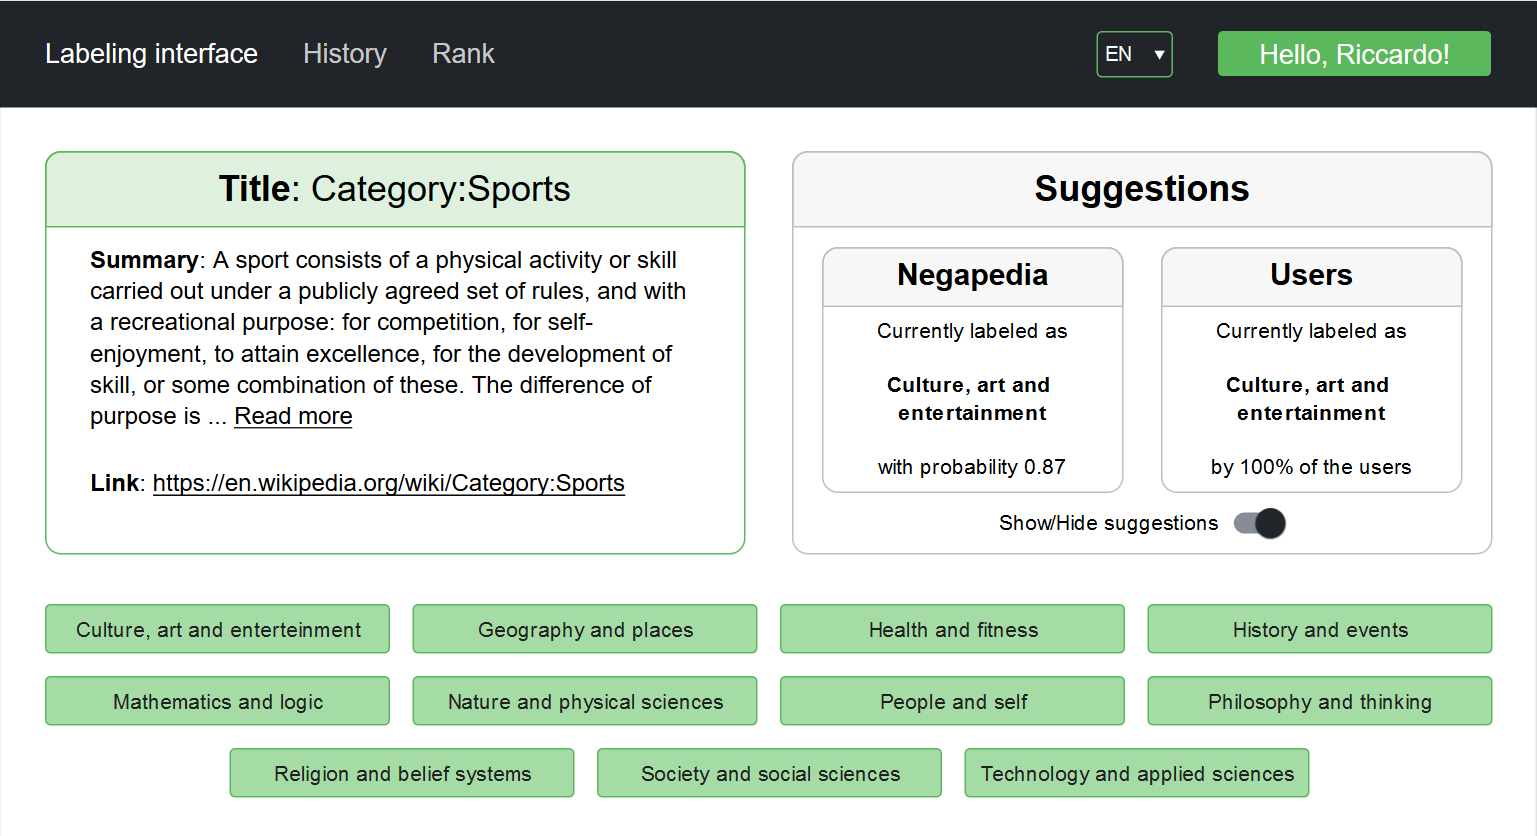
\includegraphics[height=0.735\textwidth, angle=90]{images/website.png}
            \caption{Labelling platform. Preview of the labelling interface page.}
            \label{labelling_platform_img}
        \end{figure}
        
        The structure of the platform is very simple, since it contains only three web pages (see figure \ref{labelling_platform_img}). Specifically:
        \begin{itemize}
            \item The \emph{Labelling interface} page allows a user to contribute and to classify a Wikipedia page using one of the predefined labels (see figure \ref{labelling_platform_img}).
            \item The \emph{History} page is an automatically generated page which contains the user contributions.
            \item The \emph{Rank} page displays the most active users --- i.e., those who have contributed the most.
        \end{itemize}
        \subsection{Labelling interface}
            The labelling interface is used to facilitate the manual labelling task. It can greatly improve the productivity of a user who labels Wikipedia pages manually.
            
            A user must perform some preliminary actions before being able to access the labelling interface page:
            \begin{itemize}
                \item He/She must have a registered account. Indeed, without this information many features of the platform cannot work (such as the history and rank pages). Moreover, while vandalism cannot be completely stopped, it can be limited to a certain extent: a registered account somehow helps to prevent it (only trusted users should be able to help with the labelling task).
                \item He/She must choose the preferred language (see image \ref{labelling_platform_img}). Indeed, the platform manages entries that come from several different Wikipedia versions, and a user may not be expert enough in a rare language spoken by few people (such as Venetian). 
            \end{itemize}
            
            The labelling interface page of the platform is made up of three main components (see image \ref{labelling_platform_img}):
            \begin{description}
                \item[Wikipedia page] A container that shows information about the Wikipedia page to be classified. In particular, a Wikipedia page is mainly described by its title: this is the most important information that a user have in order to understand what is the content of the page. If the title is not enough to understand what a page represents, then its summary can be used. Finally --- in case summary is absent\footnote{Pages that represent categories usually don't have the optional summary part.} and/or ambiguous --- one can navigate directly to the Wikipedia page through its hyperlink. In this way, one can check other information, such as the categories the page is linked to or which Wikipedia portal it belongs to.
                \item[Suggestions] A container that shows some suggestions --- i.e., how other sources have labeled the Wikipedia page. In particular, the aggregated information comes from Negapedia and from the database of the platform itself. With regard to the first source of information, Negapedia divides Wikipedia articles into macro categories in order to make it easier for the user to see separately the negative side of various aspects of our society, as explained in section \ref{negapedia_categories}. Therefore, such classification can help the user to do his/her choice. Moreover, the database of the labelling platform possibly contains answers given by other users: this can be helpful to the user. While asking to multiple persons the same questions may look like a waste of time, aggregated multiple answers can result in a more accurate label.
                \item[Labels] A button group that represents the arbitrary set of labels used by the learning framework to classify Wikipedia pages. The administrator of the platform can set which are the labels users can choose from, and they are dynamically showed as buttons in the labelling interface page.
            \end{description}
            
            Though having suggestions improve users' productivity, this can lead to biased labels. In other words, a suggestion may somehow \textquote{force} a user to make a specific choice, thus worsening the training set. Therefore, the user is given the option to hide the suggestions and be free to choose the option that best fits his/her thoughts, without being influenced by the output of an algorithm or by the collective knowledge of people as expressed through their aggregated opinions.
        \subsection{History}
            The history page displays users contributions. It simply lists all the pages that a user has helped to classify.
            
            \begin{figure}[h]
                \centering
                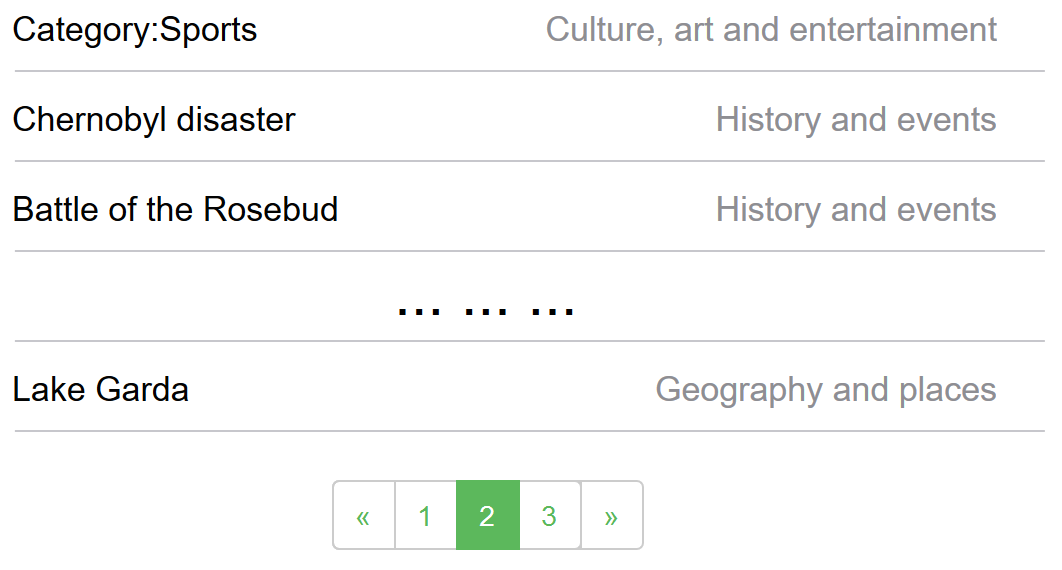
\includegraphics[width=0.7\textwidth]{images/history.png}
                \caption{User contributions in the history page of the labelling platform.}
                \label{history}
            \end{figure}
            
            In particular, each item of the history list --- i.e., each user contribution --- displays the title of the Wikipedia page that was classified and the related label associated to that specific page (see figure \ref{history}). When a users has many contributions, they are paged in order to make the section more readable and user friendly.
        \subsection{Rank}\label{rank}
            The rank page displays the most active users --- i.e., those who have contributed the most.
            
            This section of the website does not contain information which can directly help to improve the quality of the training set. Instead, it implements a basic competition among users, which is one of the simplest gamification techniques. In particular, the section displays a leaderboard, which determines who performs best in the labelling task. It has been proved that competition caused by leaderboards can increase the user's level of engagement and can consequently have a constructive effect on participation \cite{Burguillo}.
    \section{Backend}
        There is a data access layer which handles business logic and data storage, providing support to the web interface and to applications that wants to access data. It is implemented using Javascript runtime and a NoSQL database, and it provides access to some services through REST-based APIs.
        \subsection{REST-based APIs}\label{rest_api}
            The labelling interface provides very simple and basic APIs based on REST, an architectural style and approach to communications often used in web services development. They are designed to satisfy some principles described by \citeauthor{Fielding} in \cite{Fielding}:
            \begin{itemize}
                \item They are based on a client-server architecture, where the server stores and manipulates information and the client takes that information uses it.
                \item They are stateless --- i.e., calls can be made independently of one another, and each call contains all of the data necessary to complete itself successfully.
                \item They have a uniform interface that allows independent evolution of the application and the API layer itself. This simplifies the architecture, as all components follow the same rules to speak to one another.
            \end{itemize}
            
            Specifically, these APIs can be used for two main reasons:
            \begin{itemize}
                \item Anyone can gather labeled data related to one or more Wikipedia versions.
                \item Authorized applications can post new data to the platform database, in order to get it labeled.
            \end{itemize}
            Furthermore, there exists a number of less important APIs that have been built mainly to serve the web interface, and in general to get other information contained in the platform database. For example, there are APIs that allows to obtain a random unlabeled Wikipedia page (or the one with highest priority), and to get the topic names used to classify each page, etc.
            
            \subsubsection{Gather labeled data}
                This resource returns labeled data that is stored in the database.
                \begin{table}[h]
                    \begin{tabularx}{\textwidth}{|l|l|X|}
                        \hline
                        \emph{Endpoint} & \multicolumn{2}{l|}{\monospace{/labeled\_data}}  \\ \hline
                        \emph{Method} & \multicolumn{2}{l|}{\monospace{GET}} \\ \hline
                        \multirow{3}{*}{\emph{Query parameters}} & \monospace{lang} & Language code (e.g., \textquote{it} or \textquote{en}) \\ \cline{2-3} 
                                                                 & \monospace{page\_type} & Either \textquote{article} or \textquote{category} \\ \cline{2-3} 
                                                                 & \monospace{id} & Page identifier \\ \hline
                    \end{tabularx}
                \end{table}
                
                In particular, a user can optionally set some parameters through the query string of the URL. The \monospace{lang} parameter allows to specify the Wikipedia version data belongs to; the \monospace{page\_type} parameter allows to select only labeled articles or categories; finally, the \monospace{id} parameter --- which must be used together with \monospace{lang} --- indicates a specific desired page. The JSON response is made up of a number of labeled entries:
\begin{lstlisting}[basicstyle=\small]
[{"lang": "en", "id": 127, "label": "Health and fitness"},
 ...,
 {"lang": "en", "id": 245975, "label": "People and self"}]
\end{lstlisting}
            If the list contains too many results then data is sent in response as a series of \textquote{chunks}. In other words, groups of elements are sent one by one, without closing connection until the last one is passed.
            \subsubsection{Post new data}
                An application (for example, one that is using the learning framework described in chapter \ref{learning_framework}) may want to get some Wikipedia pages labeled. However, these pages may not be stored in the database yet. Therefore, the application needs a way to post new data to the labelling platform. Moreover, in case the application is a active learner, it may need to have a page labeled as soon as possible (otherwise training cannot advance): APIs allows to set the priority of each entry, thus providing a way to indicate what are the most important pages to be labeled.
                
                \begin{table}[h]
                    \begin{tabularx}{\textwidth}{|l|l|X|}
                        \hline
                        \emph{Endpoint} & \multicolumn{2}{l|}{\monospace{/data}}  \\ \hline
                        \emph{Method} & \multicolumn{2}{l|}{\monospace{POST}} \\ \hline
                        \multirow{4}{*}{\emph{Body parameters}} & \monospace{lang} & Language code (e.g., \textquote{it} or \textquote{en}) \\ \cline{2-3}
                                                                & \monospace{id} & Page identifier \\ \cline{2-3}
                                                                & \monospace{priority} & Priority (number greater than \(0\)) \\ \cline{2-3}
                                                                & \monospace{key} & API authorization key  \\ \hline
                    \end{tabularx}
                \end{table}
                
                In order to prevent vandalism and, in general, to avoid unauthorized applications to add data to the database, it is necessary to add a \monospace{key} field (though it is probably superfluous in such a setting, where there are only few trusted contributors and users).
        \subsection{Server and database implementation}
            The server has been built using Node.js\footnote{\url{http://nodejs.org/}.}, a free and open source cross-platform runtime environment for server-side programming that allows users to build network applications in Javascript. I have chosen Node.js because of its performance and portability.
            
            I have also made use of Express\footnote{\url{http://expressjs.com/}.}, a web application framework that provides simple handlers for requests with different HTTP verbs, and allows a user to add additional request processing \textquote{middleware} at any point within the request handling pipeline.
            
            Finally, I have chosen MongoDB\footnote{\url{http://mongodb.com/}.}, a free,  general purpose, document-based database. It stores data in JSON-like documents, meaning fields can vary from document to document and data structure can change over time.